\documentclass[tikz,border=3pt]{standalone}
\usepackage{tikz-feynman}
\begin{document}
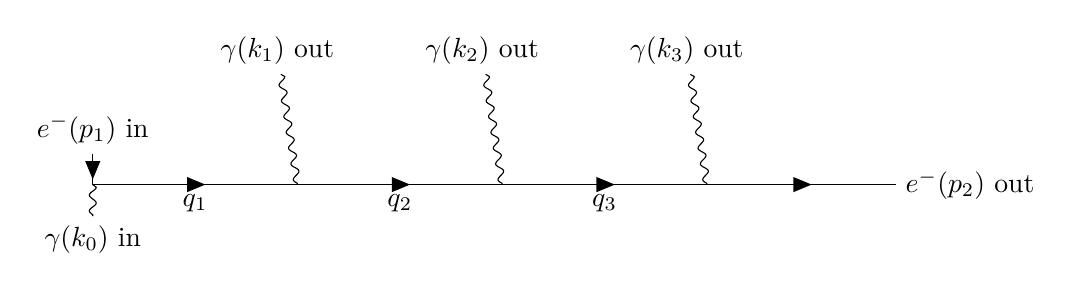
\begin{tikzpicture}
\begin{feynman}
\vertex (ein) {\(e^-(p_1)\) in};
\vertex[below=1.4cm of ein] (gin) {\(\gamma(k_0)\) in};
\vertex[right=2.4cm of ein, below=0.7cm of ein] (A);
\vertex[above right=1.4cm and 1.5cm of A] (g1) {\(\gamma(k_1)\) out};
\vertex[right=2.6cm of A] (C);
\vertex[above right=1.4cm and 1.5cm of C] (g2) {\(\gamma(k_2)\) out};
\vertex[right=2.6cm of C] (D);
\vertex[above right=1.4cm and 1.5cm of D] (g3) {\(\gamma(k_3)\) out};
\vertex[right=2.6cm of D] (B);
\vertex[above=0.7cm of B, right=2.4cm of B] (eout) {\(e^-(p_2)\) out};

\diagram* {
  (ein) -- [fermion] (A),
  (gin) -- [photon] (A),
  (A) -- [fermion, edge label'=\(q_1\)] (C),
  (C) -- [photon] (g1),
  (C) -- [fermion, edge label'=\(q_2\)] (D),
  (D) -- [photon] (g2),
  (D) -- [fermion, edge label'=\(q_3\)] (B),
  (B) -- [photon] (g3),
  (B) -- [fermion] (eout),
};
\end{feynman}
\end{tikzpicture}
\end{document}
